\documentclass{article}

\usepackage[utf8]{inputenc}
\usepackage[T1]{fontenc}
\usepackage{fourier}
%\usepackage[latin1]{inputenc}
\usepackage[spanish]{babel}

\usepackage[thinlines]{easytable}
\usepackage{diagbox}
\usepackage{multirow}


\usepackage[protrusion=true,expansion=true]{microtype}	
\usepackage{amsmath,amsfonts,amsthm} % Math packages
\usepackage{amssymb}
\usepackage[pdftex]{graphicx}	
\usepackage{url}
\usepackage{tikz}
\usepackage{setspace}
\usepackage{import}
\usepackage{float}
\usepackage{graphicx}
\pagenumbering{arabic}
%margenes 
\usepackage{geometry}
 \geometry{
 a4paper,
 left=19mm,
 right=19mm,
 top=19mm,
 bottom=42mm,
 }

% %%% Custom sectioning
\usepackage{sectsty}
%\allsectionsfont{\normalfont \scshape}


%%% Custom headers/footers (fancyhdr package)
\usepackage{fancyhdr}
\pagestyle{fancyplain}
\fancyhead{}											% No page header
\fancyfoot[L]{}											% Empty 
\fancyfoot[C]{}											% Empty
\fancyfoot[R]{\thepage}									% Pagenumbering
\renewcommand{\headrulewidth}{0pt}			% Remove header underlines
\renewcommand{\footrulewidth}{0pt}				% Remove footer underlines
\setlength{\headheight}{13.6pt}


%%% Equation and float numbering
\numberwithin{equation}{section}		% Equationnumbering: section.eq#
\numberwithin{figure}{section}			% Figurenumbering: section.fig#
\numberwithin{table}{section}				% Tablenumbering: section.tab#


%%% Maketitle metadata
\newcommand{\horrule}[1]{\rule{\linewidth}{#1}} 	% Horizontal rule

\begin{document}

\onehalfspacing

\begin{titlepage}
    
\newcommand{\HRule}{\rule{\linewidth}{0.5mm}} % Defines a new command for the horizontal lines, change thickness here
    
\center % Center everything on the page
     
%----------------------------------------------------------------------------------------
%	HEADING SECTIONS
%----------------------------------------------------------------------------------------
    
\textsc{\LARGE Instituto Tecnológico de Buenos Aires}\\[2cm] % Name of your university/college
\textsc{\Large 22.42 Laboratorio de Electrónica}\\[1.5cm] % Major heading such as course name
\textsc{\large Trabajo Práctico N° 2}\\[0.5cm] % Minor heading such as course title
    
%----------------------------------------------------------------------------------------
%	TITLE SECTION
%----------------------------------------------------------------------------------------
    
\HRule \\[0.5cm]
{ \huge \bfseries Osciloscopios/ Analizador de Impedancias/ \\Circuitos RLC}\\[0.4cm] % Title of your document
\HRule \\[2cm]
     
%----------------------------------------------------------------------------------------
%	AUTHOR SECTION
%----------------------------------------------------------------------------------------
    
\begin{minipage}{0.4\textwidth}
\begin{flushleft} \large
\emph{Grupo 5:}\\		%names
[.3cm]
Nicolás \textsc{De León}\\
Leg. 57232\\ 
[.3cm]
Tomás \textsc{Vigón}\\
Leg. 57327\\ 
[.3cm]
Benjamín \textsc{Lin}\\
Leg. 57242 \\ 
[.3cm]
Lucero Guadalupe \textsc{Fernandez}\\
Leg. 57485\\ 
[.3cm]
\end{flushleft}
\end{minipage}
~
\begin{minipage}{0.4\textwidth}
\begin{flushright} \large
\emph{Profesor:} \\
[.3cm]
Pablo  \textsc{Cossutta}\\ % Supervisor's Name
Alejandra \textsc{Weill} \\% Supervisor's Name
Matías  \textsc{Salvati} % Supervisor's Name
\end{flushright}
\end{minipage}\\[2cm]
    
%----------------------------------------------------------------------------------------
%	DATE SECTION
%----------------------------------------------------------------------------------------
    
\vfill
{\large Entregado: 25 de Septiembre de 2018}\\[2cm]
    
\vfill 
    
\end{titlepage}

\section{Medicion de Componentes con Analizador de Impedancia}


\section{Respuesta del Circuito LRC}

Se armo el circuito LRC representado en la figura \ref{fig:LRC1}, cuyos valores nominales son $L=1mH$ para la bobina y $C=8.2nF$ para el capacitor. Con el uso de un Buffer en la entrada se evitar impedancia del generador y que se cargue el generador, provocando un funcionamiento incorrecto durante las mediciones.

\begin{figure}[h!]
\centering
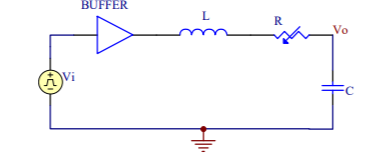
\includegraphics[scale=0.5]{lrcCircuito.png}
\caption{Circuito LRC armado}
\label{fig:LRC1}
\end{figure}

La ecuacion característica del circuito es $\frac{s^2}{\omega_0^2}+s\frac{2\xi}{\omega_0}+1$, donde $\omega_0 = \frac{1}{\sqrt{LC}}$ y $\xi = \frac{\omega_0RC}{2}$. Calculado la frecuencia de resonancia $f_0=55.5kHz$ y teniendo en cuenta el valor de $\xi = 0.19$ hallamos el valor de la resistencia $R = 130\Omega$. Cabe notar que el factor de calidad $Q = \frac{1}{2\xi}$ por lo que resulta en este caso $Q = 2.6$, por lo tanto se trataria de un circuito sub-amortiguado. 

\subsection{Respuesta al Escalon}

Exitando el circuito con una onda cuadrada de $V_i = 0.5V_{pp}$ y una frecuencia de $f = 5.5kHz$ obteniendo la siguiente respuesta:

\begin{figure}[h!]
\centering
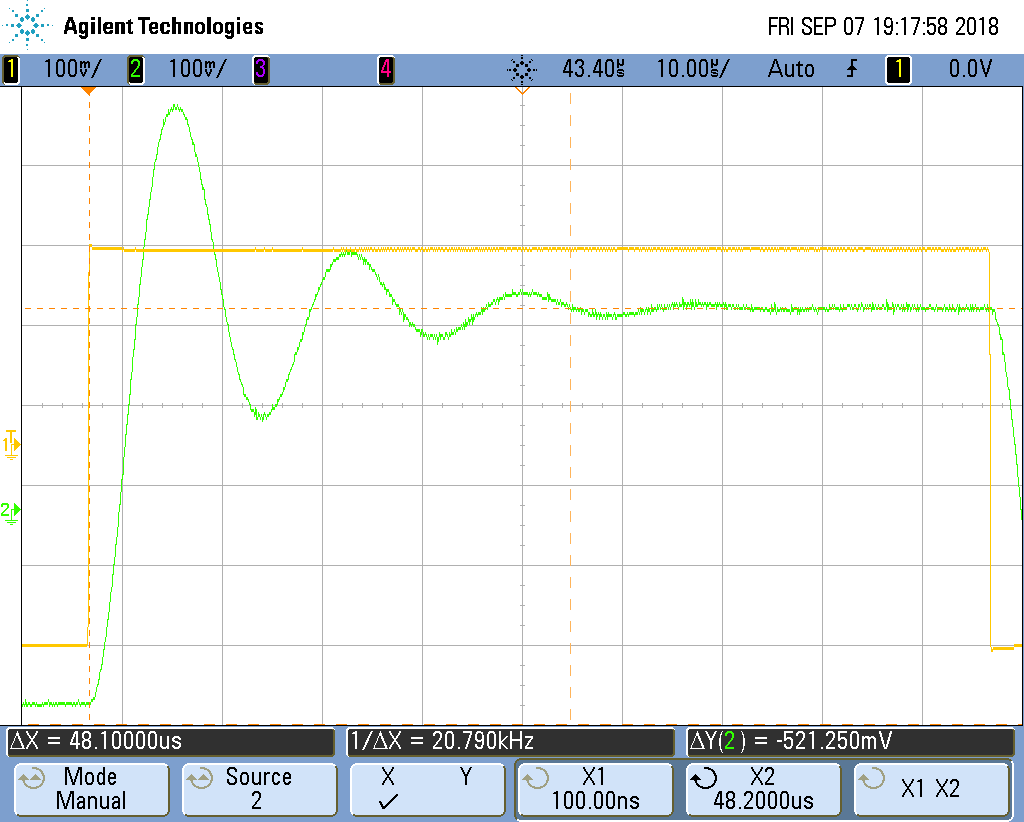
\includegraphics[scale=0.25]{LRC2a.png}
\caption{Respuesta al escalon}
\label{fig:LRC2}
\end{figure}

De tal manera que se obtuvo un sobrepico de $M_p = 757mV$, un tiempo de establecimiento del $5\%$ $t_s = 47.6{\mu}s$ y su frecuencia de oscilacion $f_t = 56.2kHz$. Como criterio para la medicion del tiempo de establecimie se tomo la diferencia de tiempo desde la exitacion de la señal cuadrada y el tercer sobrepico de la oscilacion. Notamos que la señal de salida tiene comportamiento de una oscilacion subamortiguada, donde el capacitor y la inductancia en seria actuan como un oscilador y la resistencia actua como dicipador de energia reduciendo asi la amplitud de la oscilacion.

Se obtuvo la respuesta analitica del circuito partiendo de la ecuacion: $$\frac{V_c''(t)}{\omega_0^2} + \frac{V_c'(t) 2\xi}{\omega_0} + V_c(t) =  0.5u(t)$$ tal que las condiciones iniciales son nulas. Con el uso de la transformada de Laplace llegamos a $V_c(s) = \frac{0.5}{s(\frac{s^2}{\omega_0^2}+\frac{s2\xi}{\omega_0}+1)}$ por lo que su antitransformada es equivalente a:$$V_c(t) = 0.5\left(1-\frac{e^{-\xi\omega_0t}}{\sqrt{1-\xi^2}}\sin{\left(\omega_0\sqrt{1-\xi^2}t+\arctg{\frac{\sqrt{{1-\xi^2}}}{\xi}}\right)}\right)$$ 
De esta manera se podra derivar $V_c(t)$ y hallar el punto critico, es decir el sobrepico de la funcion que tiene forma $t_p=\frac{\pi}{\omega_0\sqrt{1-\xi^2}}$, lo que resulta en este caso $t_p=9.18{\mu}s$ y su correspondiente valor $M_p=772mV$. Como describe la ecuacion la frecuencia de oscilación es $f_t= \frac{\omega_0\sqrt{1-\xi^2}}{2\pi} = 54.5kHz$. Por ultimo el tiempo de establecimiento de la señal la aproximamos con $t_s=\frac{\pi}{\xi\omega_0}$ que obtenemos $t_s = 47.42{\mu}s$

Comparando los resultados analiticos y experimentales, los resultados estan en el mismo orden si bien existen diferencias las cuales pueden ser debido a errores accidentales en las mediciones y aproximaciones en los calculos teoricos. 

\subsection{Effecto de la frecuencia en el circuito LRC}
Se


\end{document}
